% !Mode:: "TeX:UTF-8"
\chapter{实验结果}
\section{灰度化}
结果如图4.1
\begin{figure}[h]
	\centering
	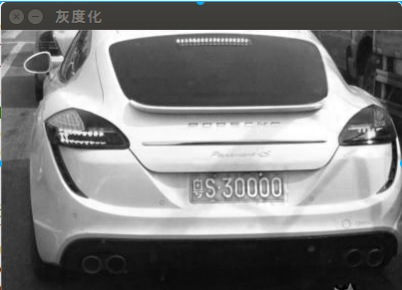
\includegraphics[scale=0.5]{figures/10.png}
	\caption{灰度化}
	\label{fig:2}
\end{figure}

\section{高斯滤波}
结果如图4.2
\begin{figure}[h]
	\centering
	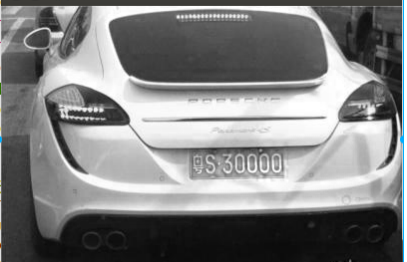
\includegraphics[scale=0.5]{figures/11.png}
	\caption{高斯滤波}
	\label{fig:2}
\end{figure}

\section{Sobol算子}
结果如图4.3
\begin{figure}[h]
	\centering
	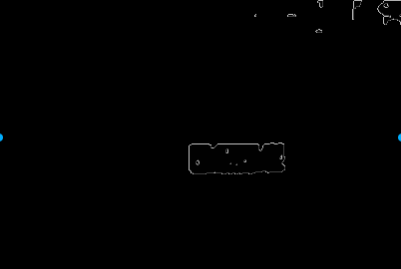
\includegraphics[scale=0.5]{figures/12.png}
	\caption{Sobol}
	\label{fig:2}
\end{figure}

\section{二值化}
结果如图4.4
\begin{figure}[h]
	\centering
	
\includegraphics[scale=0.5]{figures/13.png}
	\caption{二值化}
	\label{fig:2}
\end{figure}

\section{闭运算}
结果如图4.5
\begin{figure}[h]
	\centering
	
\includegraphics[scale=0.5]{figures/14.png}
	\caption{闭运算}
	\label{fig:2}
\end{figure}

\section{定位}
\begin{enumerate}
	\item 简单车牌定位,结果如图4.6
	\item 复杂车牌定位,结果如图4.7
\end{enumerate}

\begin{figure}[h]
	\centering
	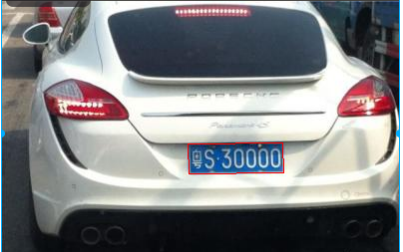
\includegraphics[scale=0.5]{figures/15.png}
	\caption{简单定位}
	\label{fig:2}
\end{figure}

\begin{figure}[h]
	\centering
	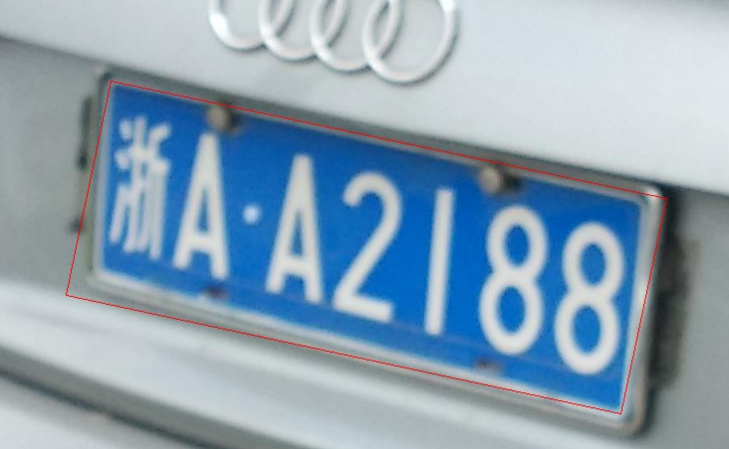
\includegraphics[scale=0.5]{figures/16.png}
	\caption{复杂定位}
	\label{fig:2}
\end{figure}

\section{字符分割}
结果如图4.8
\begin{figure}[h]
	\centering
	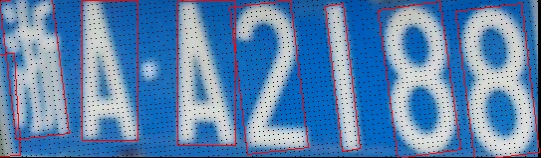
\includegraphics[scale=0.5]{figures/17.png}
	\caption{分割}
	\label{fig:2}
\end{figure}